The \nameref{ch:problem} mainly described the needs which the Flashmap System might be able to accomodate, and on page~\pageref{sec:intro_flashmap} generic features of such a system are described. Although the term Flashmap System is intended for describing any system including these features, when having to evaluate the idea one has to evaluate one or multiple specific implementations of that idea. Therefore, this part specifies the design features of the specific tool developed within this project, along with arguments in favour of and against these choices and their considerations, and the process with which they are incorporated within the tool itself. The design process is based on the Generic Model \cite{genericmodel}, which is displayed in figure~\ref{fig:genericmodel}.

\begin{figure}[h]
    \centering
    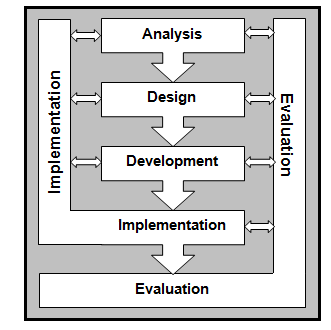
\includegraphics[width=0.5\textwidth]{img/genericmodel}
    \caption{The generic model by \protect\citeA{genericmodel}\label{fig:genericmodel}}
\end{figure}

The first chapter, \nameref{ch:analysis} on page~\pageref{ch:analysis}, describes the design implications stemming from the context, learner, and learning task of this project. The next chapter, \nameref{ch:frameworks} on page~\pageref{ch:frameworks}, describes implications from theoretical design frameworks relevant to the design of the flashcard and flashmap system. Finally, the \nameref{ch:software} chapter on page~\pageref{ch:software} describes the actual implementation of the software following from the design implications of the previous chapters.
